
%(BEGIN_QUESTION)
% Copyright 2007, Tony R. Kuphaldt, released under the Creative Commons Attribution License (v 1.0)
% This means you may do almost anything with this work of mine, so long as you give me proper credit

Shown here is the response of a proportional+integral controller to a step-change in setpoint (with a constant process variable).  Calculate the controller's proportional and integral constant settings, based on what you see in the graph.  Express your answer for the integral constant both in units of ``repeats per minute'' and ``minutes per repeat.''  Also, determine whether this controller is direct or reverse acting, and mark the features of the output plot corresponding to proportional action and to integral action.
  
$$\includegraphics[width=15.5cm]{i01602x01.eps}$$

The time scale on the chart is minutes:seconds, and the PI algorithm is as follows:

$$m = K_p \left( e + {1 \over \tau_i} \int e \> dt \right) + b$$

\noindent
Where,

$m$ = Controller output (manipulated variable)

$K_p$ = Gain

$e$ = Error signal (SP$-$PV or PV$-$SP)

$\tau_i$ = Integral time constant

$b$ = Bias

\vskip 10pt

\vskip 20pt \vbox{\hrule \hbox{\strut \vrule{} {\bf Suggestions for Socratic discussion} \vrule} \hrule}

\begin{itemize}
\item{} When analyzing the output trend of a PI controller, the definition of the reset time constant as being ``the number of minutes required to per repeat proportional action'' is most useful.  Identify the magnitude of proportional action in response to the PV step-change, and then explain how this value is helpful in identifying $\tau_i$.
\item{} If you really saw this type of response on a process controller trend (chart recorder), what might you suspect about the system?  Hint: this type of trend is definitely {\it not} normal for a properly functioning control system!
\end{itemize}

\underbar{file i01602}
%(END_QUESTION)





%(BEGIN_ANSWER)

Controller action = {\it direct}

\vskip 10pt

Gain constant = 1, or 100\% proportional band

\vskip 10pt

Integral constant = 0.25 repeats per minute ($\tau_i$), or 4 minutes per repeat ($K_i$)

%(END_ANSWER)





%(BEGIN_NOTES)

We know this controller's action is {\it direct} because the output decreases as the setpoint (SP) increases.  That is to say, the output would decrease if the process variable input (PV) were to decrease.  

This controller's gain is calculated by the ratio of the output step-change magnitude to the input step-change magnitude: in this case, a 20\% output step-change is caused by a 20\% input step-change, for a gain of 1.  Reciprocating this value, we have a proportional band of 100\%.

Finally, we see that over a minute's period of time, the integral action causes the output to drift another 5\%.  This is only 1/4 that of the proportional action's response, so the integral constant value is 1/4 repeat per minute.  Reciprocating, we get 4 minutes per repeat.
 
\vskip 10pt

What is wrong with this control system, as indicated by the trend?  The process variable seems completely unresponsive to the output signal's change!  It would appear the final control element has been bypassed or disengaged somehow.  Do not think that this indicates a controller in the manual mode.  A controller left in ``manual'' would not generate any change in output signal corresponding to changes in either the PV or SP signals.  In other words, a controller in the ``manual'' mode would hold a constant output signal level no matter what happens to the PV or SP.

%INDEX% Control, proportional + integral: graphing controller response

%(END_NOTES)


